
\vspace{-1.5cm}
\section*{Model}
\vspace{-0.2cm}

Motivated from the observed anisotropy in axonal morphology (Fig.~\ref{fig:morphaniso}) we formulate the \textit{anisotropic network model}: $N=1000$ neurons are distributed uniformly on a square of length \SI{296}{\micro\meter}. Each neuron is assigned a random direction $\alpha \in [0,2\pi)$ and connections are established to target neurons lying within in a corridor of width $w=\text{\SI{74.6}{\micro\meter}}$ (Fig.~\ref{fig:4nets}A). Here, the width $w$ was tuned to obtain a network connection density of $p=11.6$ as found in \cite{Song2005}.

\begin{center}\vspace{0.3cm}
  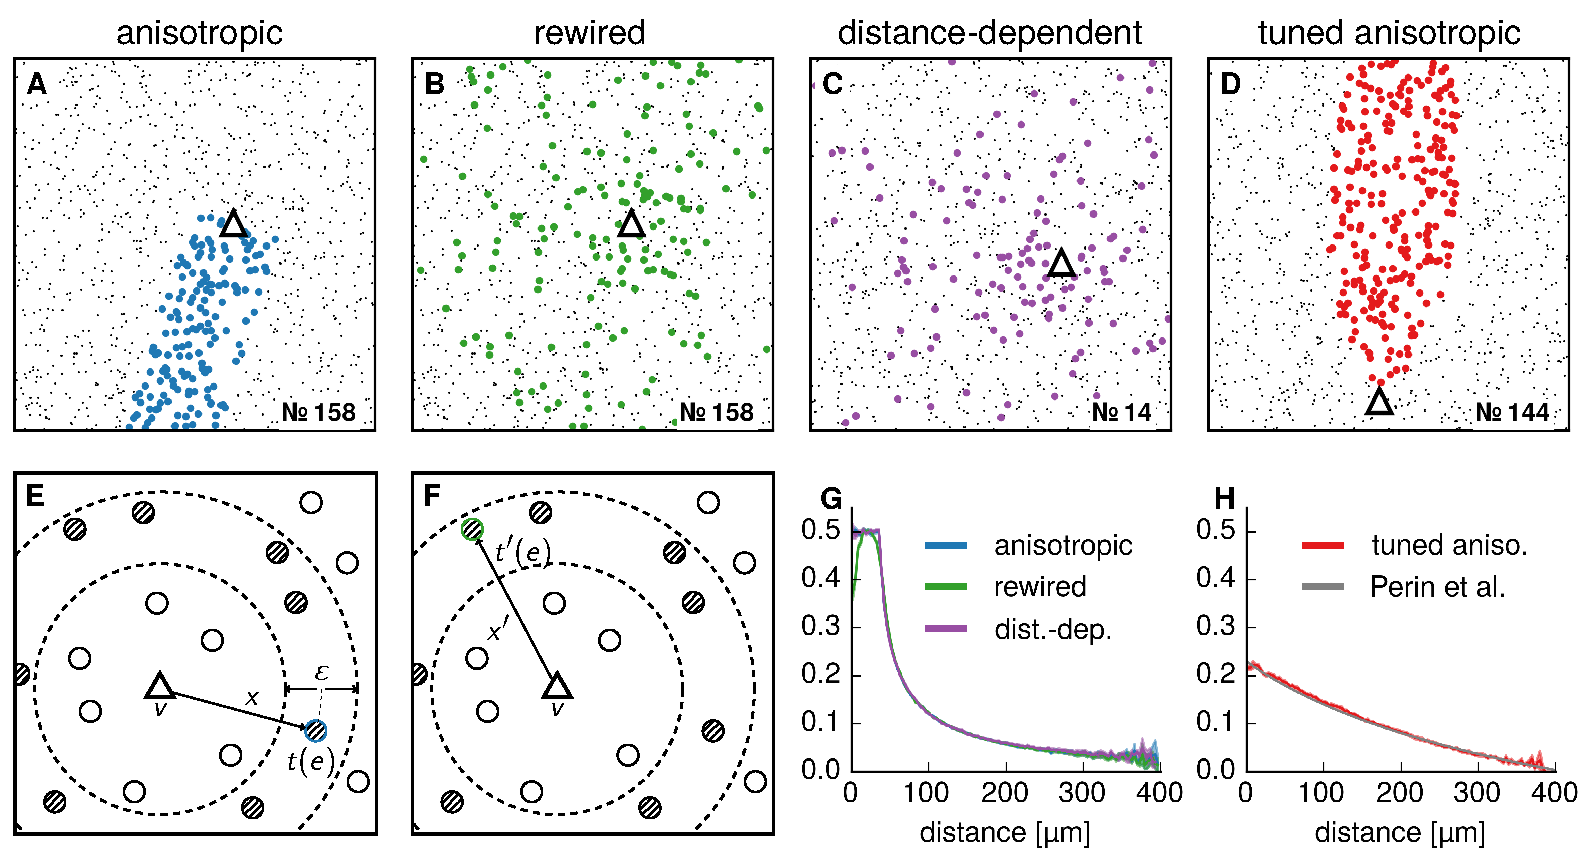
\includegraphics[width=\columnwidth]{%
    /home/fh/sci/rsc/aniso_netw/pub/arxiv18/figures/4_network_models/4_network_models.pdf}
  \captionof{figure}{Network models. \textbf{A-D} Targets of a single neuron (Id in bottom right corner) for the different network models \textbf{E-F} Rewiring algorithm. \textbf{G-H} Distance-dependent connection probabilities.}
  \label{fig:4nets}
\end{center}\vspace{2cm}

The \textit{rewired network} (Fig.~\ref{fig:4nets}B) is obtained from the anisotropic network by randomly picking new targets that differ in distance to the source neuron maximally by $\epsilon$ from the original target (Fig.~\ref{fig:4nets}E-F). The \textit{distance-dependent network} (Fig.~\ref{fig:4nets}C) is a randomly connected graph where the probability of a connection to exist depends on the distance between the nodes, using for example the profile of the anisotropic network (Fig.~\ref{fig:4nets}G). Finally, the \textit{tuned anisotropic network} (Fig.~\ref{fig:4nets}D) is similar to the anisotropic network with the difference that the corridor is shaped in such a way that the distance-dependent connection probability found in \cite{Perin2011} is obtained in the network (Fig.~\ref{fig:4nets}H).



